
\documentclass[11pt]{article}\usepackage[]{graphicx}\usepackage[]{color}
%% maxwidth is the original width if it is less than linewidth
%% otherwise use linewidth (to make sure the graphics do not exceed the margin)
\makeatletter
\def\maxwidth{ %
  \ifdim\Gin@nat@width>\linewidth
    \linewidth
  \else
    \Gin@nat@width
  \fi
}
\makeatother

\definecolor{fgcolor}{rgb}{0.345, 0.345, 0.345}
\newcommand{\hlnum}[1]{\textcolor[rgb]{0.686,0.059,0.569}{#1}}%
\newcommand{\hlstr}[1]{\textcolor[rgb]{0.192,0.494,0.8}{#1}}%
\newcommand{\hlcom}[1]{\textcolor[rgb]{0.678,0.584,0.686}{\textit{#1}}}%
\newcommand{\hlopt}[1]{\textcolor[rgb]{0,0,0}{#1}}%
\newcommand{\hlstd}[1]{\textcolor[rgb]{0.345,0.345,0.345}{#1}}%
\newcommand{\hlkwa}[1]{\textcolor[rgb]{0.161,0.373,0.58}{\textbf{#1}}}%
\newcommand{\hlkwb}[1]{\textcolor[rgb]{0.69,0.353,0.396}{#1}}%
\newcommand{\hlkwc}[1]{\textcolor[rgb]{0.333,0.667,0.333}{#1}}%
\newcommand{\hlkwd}[1]{\textcolor[rgb]{0.737,0.353,0.396}{\textbf{#1}}}%

\usepackage{framed}
\makeatletter
\newenvironment{kframe}{%
 \def\at@end@of@kframe{}%
 \ifinner\ifhmode%
  \def\at@end@of@kframe{\end{minipage}}%
  \begin{minipage}{\columnwidth}%
 \fi\fi%
 \def\FrameCommand##1{\hskip\@totalleftmargin \hskip-\fboxsep
 \colorbox{shadecolor}{##1}\hskip-\fboxsep
     % There is no \\@totalrightmargin, so:
     \hskip-\linewidth \hskip-\@totalleftmargin \hskip\columnwidth}%
 \MakeFramed {\advance\hsize-\width
   \@totalleftmargin\z@ \linewidth\hsize
   \@setminipage}}%
 {\par\unskip\endMakeFramed%
 \at@end@of@kframe}
\makeatother

\definecolor{shadecolor}{rgb}{.97, .97, .97}
\definecolor{messagecolor}{rgb}{0, 0, 0}
\definecolor{warningcolor}{rgb}{1, 0, 1}
\definecolor{errorcolor}{rgb}{1, 0, 0}
\newenvironment{knitrout}{}{} % an empty environment to be redefined in TeX

\usepackage{alltt}

% margins, size, formatting

\oddsidemargin=0in
\evensidemargin=0in
\topmargin=0in
\textwidth=6.5in
\textheight=9.5in
\parindent = 0 in
\pagestyle{plain}

    \usepackage[
    bottom = 2.50cm]{geometry}

\usepackage{amsmath,amssymb,amsthm, amsfonts}
\usepackage{array}
\usepackage{fancyhdr}
%\pagestyle{plain}
\pagestyle{fancy}
%\usepackage{listings}
%\usepackage{inconsolata}

\lhead{\textbf{Group 3: Data Analysis\\ Spring 2014}}
\rhead{\textbf{Nick Cummings, Liza Nicoll \\ Emily Ramos and Yiding Zhang}}
\cfoot{}
\IfFileExists{upquote.sty}{\usepackage{upquote}}{}

\begin{document}
%\SweaveOpts{concordance=TRUE}

\section{Introduction} %Emily

The dataset we will be using for our group analysis is ``Exploring Relationships in Body Dimensions". This dataset contains information on 21 body dimension measurements (including skeletal measurements and girth measurments) as well as age, weight, height and gender from 507 physically active men and women within the normal weight range. Most of these individuals are in their 20s and 30s. The initial reason the data was collected was to determine how well weight could be predicted between body build, weight, and girths. \\ 

This analysis will include our group analysis: summary of the dataset, our hypothesis, the base model we will be using, applications of the data and model, and our individual analyses: regression trees, model selection, resampling inference, bootstrapping, logistic regression and Ada-boosting.

%------------------------------------------------
\section{Group Analysis} 





%------------------------------------------------

\subsection{Summary of the Dataset}

%-------------------------------------------------
\\

\textbf{Variables in the Dataset}\\ %Emily

There are a total of 25 variables.\\

Skeletal measurements include: biacromial diameter, pelvic breadth, bitrochanteric diameter, chest depth, chest diameter, elbow diameter, wrist diameter, knee and ankle diameter. Note that elbow, wrist, knee and ankle measurements are the sum of the two ankle diameters.\\

Girth measurements include: shoulder, chest, waist, navel, hip, thigh, flexed bicep, extended forearm, knee, calf maximum, ankle minimum and wrist minimum. Note, for thigh, bicep, forearm, knee, calf, ankle and wrist girth measurments the average of both body parts was taken.\\

Other measurements include: age, weight, height and gender (male= 1 and femal = 0).\\

%------------------------------------------------

\newpage

\textbf{Weight}\\ %Liza
   
Weight was measured for 507 physically active individuals - 247 men and 260 women. The distribution ranged from 42 kilograms to 116.4 kilograms. The mean weight and quartiles was signifigantly higher for men than women. We observe several outliers in the upper end of the range for both men and women. This may be due to the fact that the population sampled included a number of highly physicaly fit individuals with higher than average muscle mass.

\begin{knitrout}
\definecolor{shadecolor}{rgb}{0.969, 0.969, 0.969}\color{fgcolor}
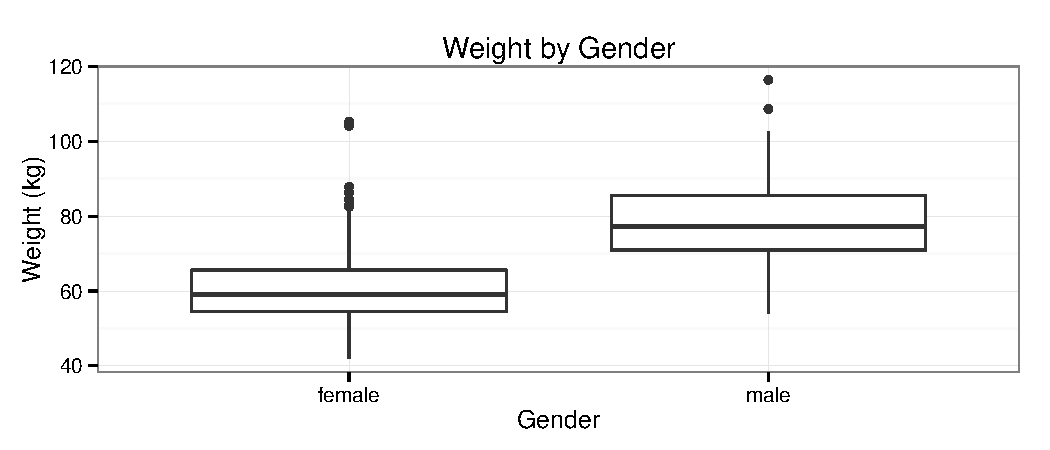
\includegraphics[width=\maxwidth]{figure/weight_plot} 

\end{knitrout}


%------------------------------------------------

\newpage

\textbf{Bitrochanteric Diameter and Hip Girth}\\ %Liza
 
Bitrochanteric diameter is the distance between the outer points of the hips and hip girth is the circumference of the hip area measured at the level of the bitrochanteric diameter. The density distributions for both measures are normally distributed (though hip girth is skewed slightly right) and very similar in distribution for both men and women. A scatter plot of hip girth vs. weight suggests that weight increases linerally with increase in hip girth.

\begin{knitrout}
\definecolor{shadecolor}{rgb}{0.969, 0.969, 0.969}\color{fgcolor}
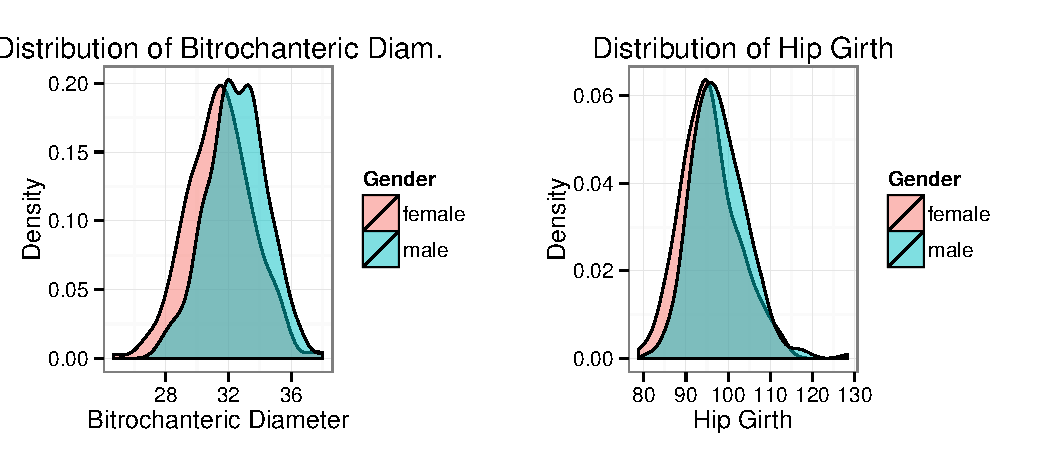
\includegraphics[width=\maxwidth]{figure/hip_plots} 

\end{knitrout}



\begin{knitrout}
\definecolor{shadecolor}{rgb}{0.969, 0.969, 0.969}\color{fgcolor}
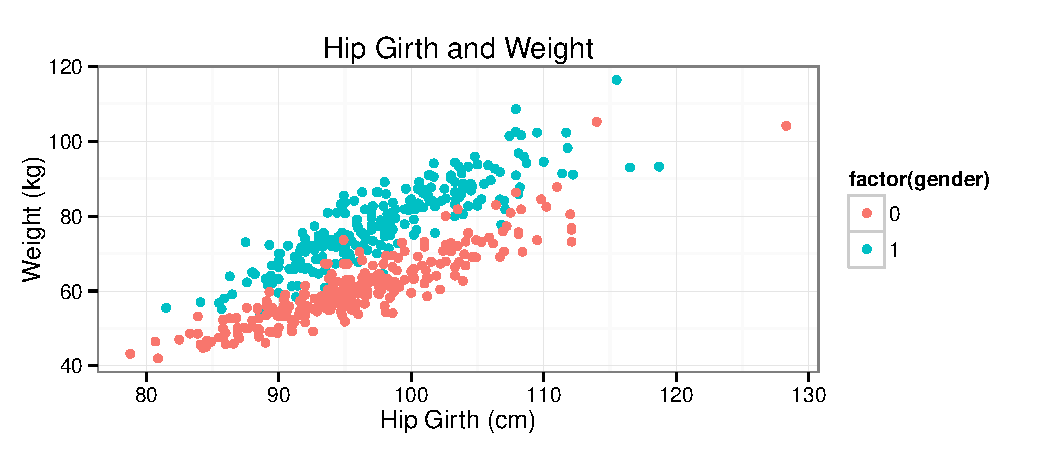
\includegraphics[width=\maxwidth]{figure/hipgirth_plot} 

\end{knitrout}


%------------------------------------------------

\newpage

\textbf{Chest and Shoulder}\\ %Liza
   
Chest girth was measured at the nipple line in males and just above breast tissue in females at mid-expiration and shoulder girth was measured over deltoid muscles in both males and females. The density distributions for the two variables are quite similar. Women have narrower, though slightly skeewed, distribution with a much lower mean than that of the men. The scatterplots are also similar in that the regression lines for men and women are nearly identical, indicating that weight increases linearly with increase in shoulder girth, independant of gender.

\begin{knitrout}
\definecolor{shadecolor}{rgb}{0.969, 0.969, 0.969}\color{fgcolor}
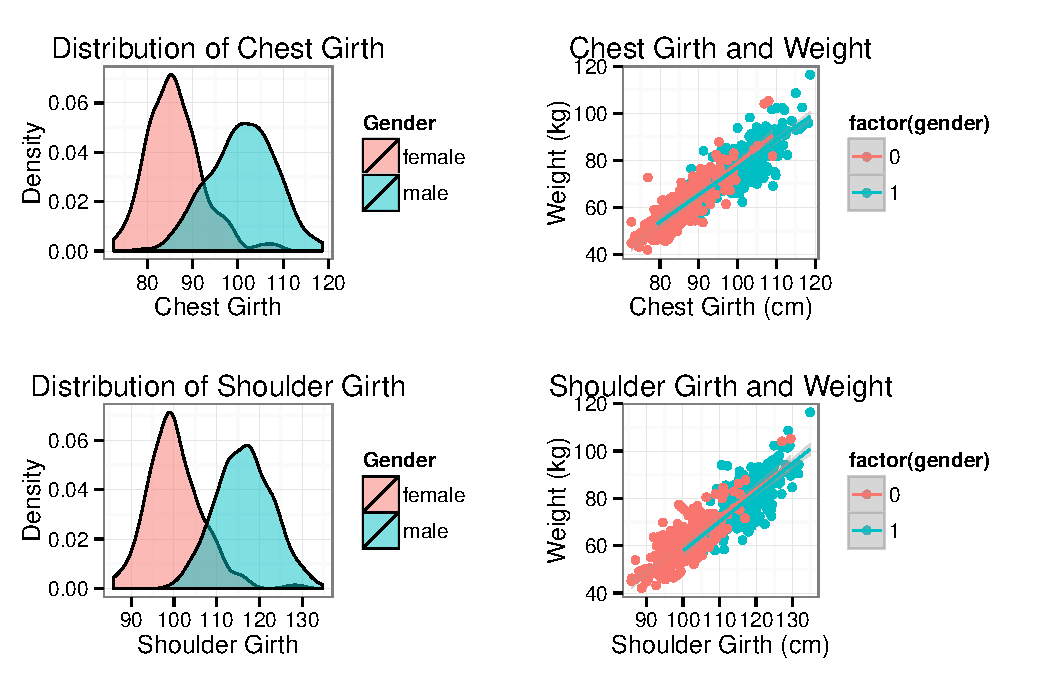
\includegraphics[width=\maxwidth]{figure/chest_plots} 

\end{knitrout}


%------------------------------------------------

\newpage

\textbf{Wrist and Navel}\\ %Liza
   
Wrist minimum girth is an average of right and left girths and navel (or abdominal) girth was measured at umbilicus and the iliac crest, using the iliac crest as a landmark. Wrist girth is bimodally distributed, but when divided into male and female, the distributions are normal with some outliers at the high end of the range for females. The distributions for navel girth is normal and remarkably similar for males and females. The scatterplot of navel girth against weight shows a linear relationship with weight increasing with increased naval girth.

\begin{knitrout}
\definecolor{shadecolor}{rgb}{0.969, 0.969, 0.969}\color{fgcolor}
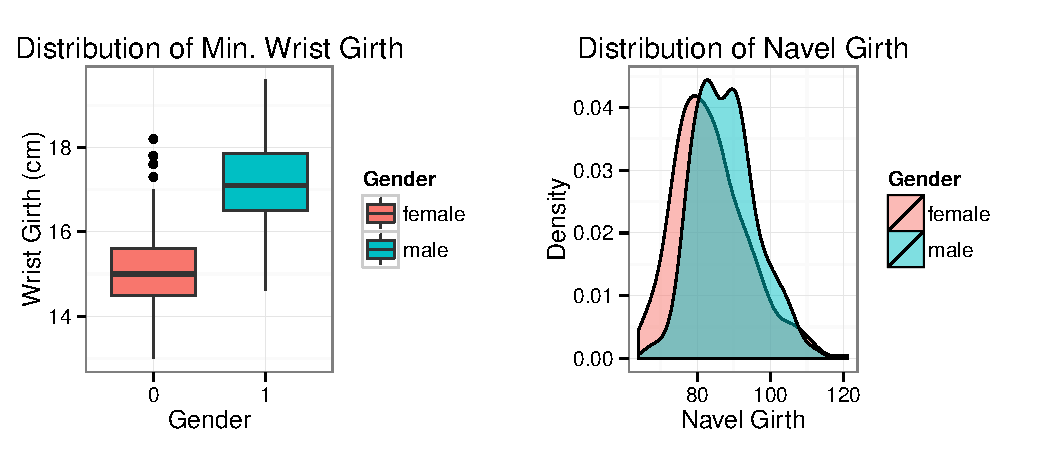
\includegraphics[width=\maxwidth]{figure/navel_plots} 

\end{knitrout}


\begin{knitrout}
\definecolor{shadecolor}{rgb}{0.969, 0.969, 0.969}\color{fgcolor}
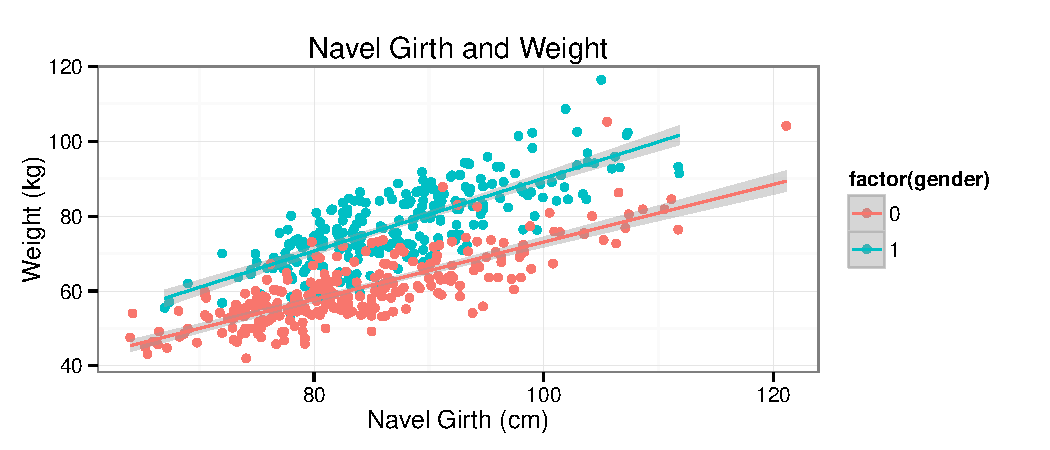
\includegraphics[width=\maxwidth]{figure/navelgirth_plot} 

\end{knitrout}


\newpage

\textbf{Age and Weight}\\ %Yiding

Since our dataset contains information on \textit{mostly} individuals in their 20s and 30s, we should check how age and weight intereact in our data before conducting analysis on weight. The mean age is 30, the youngest subject is 18 and the oldes subject is 67. The first plot shows that age is unevenly distributed, i.e left skewed. Most of the subjects are physically active young individuals. Since we have this skewness of data, we seperate the data into two subsets- young and middle age to see how weight interacts in these subsets. The weight of young and middle age groups are generally normally distributed and are remarkably similar. This shows that, although our ages are skewed, we can apply this analysis to physically active individuals of all ages.

\begin{knitrout}
\definecolor{shadecolor}{rgb}{0.969, 0.969, 0.969}\color{fgcolor}
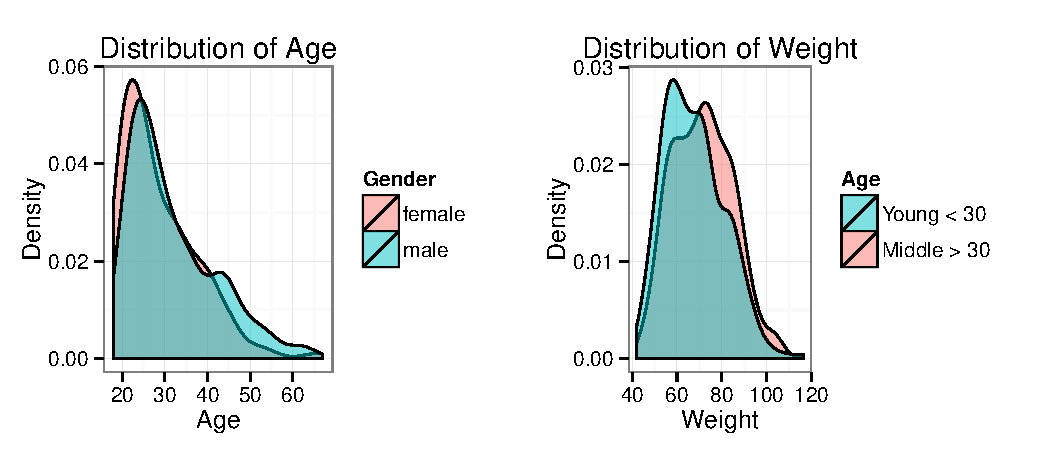
\includegraphics[width=\maxwidth]{figure/unnamed-chunk-1} 

\end{knitrout}



%------------------------------------------------

\subsection{Initial Multiple Linear Regression Model} 

%------------------------------------------------

\subsubsection{Hypothesises}%Yiding

%------------------------------------------------

\textbf{Weight}\\ 
In two ways one can get a plausible model: statistical analysis and experience. Upon initial exploration, we notice that several variables have high $p$-values, such as navel girth and flexed bicep. From a statistical perspective, these variables may be considerated as non-significant variables; however, in the paper, the author use the initial model with a adjusted $R^2 = 0.946$ and state that students could apply it to predict their weight. The model is long and includes several non-significant variables. The author also introduces another model which can be used as the standard healthy body weight predict model, but the model includes two implausible variables: ankle and wrist. On the one hand, the model is well fitted with strong significance for all variables and $R^2$ of 0.887; on the other hand, the model is too simple and also includes two implausible vaiables.\\

As we know, the majority of a persons body weight accumulates in the middle of body(beneath head and above knee). Given this information, one can predict if a person is overweight, strong, normal, or thin. Thus, we could directly and empirically add variables that make a large contribution to the weight to the model. For example, we could include shoulder girth, chest diam, waist, hip and thigh girth. The model would become:\\

weight$_i = \beta_0 + \beta_1$ shoulder$_i + \beta_2$ chest.diam$_i + \beta_3$ waist$_i + \beta_4$ hip$_i + \beta_5$ thigh$_i$ \\

We now have significant $p$-values for all of them ($<0.001$) and adjusted $R^2 = 0.853$. \\

We can obtain a ``well fitted" model from both methods and each of them has their strengths, but the question is which one is better and more meaningful. Thus, we must  take consideration of both methods and then get a good-fitting, meaningful model.\\

\textbf{Gender}\\
As we discuss in the section \textbf{Summary of the Dataset}, we can easily disinguish the difference of dimensions between male and female. Some of them do have obviouse difference such as chest girth and shoulder girth, some of do not. So we assume that when the weight model been divided into two groups---male and female, the model would present changes in each $\beta$ and become more accurate.\\

Now that gender would make the fitted model different, which would make the most accurate prediction, the fact that the subject is male or female? In the paper, the author mentions that:
\begin{quotation}
Most useful to this determination of gender are the pelvis and the skull... Using biacromial diameter as the only classifier variable, quadratic discriminant analysis with cross-validation correctly classified gender 89.3\% of the time with the 507 cases in the dataset. (Nickell and Fischer 1999; Innes 2000; Owen 2000)
\end{quotation}
We suppose that after division of gender the variables that have significant changes of their $\beta$ would be the variables that make the classification for gender accurate.\\

\subsubsection{Initial Multiple Linear Regression Model} % Emily

The initial model we are interested in fitting is of the form:\\

weight$_i = \beta_0 + \beta_1$ chest.diam$_{i} + \beta_2$ chest.dep$_{i} + \beta_3$ bitro.diam$_{i} + \beta_4$ wrist.min$_{i}$ + \beta_5$ ankle.min$_{i} + \beta_6$ height$_{i}$ \\

This model was chosen based on the idea that these variables remain constant over a persons adult years. Thus, a person can input these measurements and determine their weight. Recall, the initial objective of the study was to determine how well weight could be predicted. Although the paper mentioned multiple models one could use, we chose this as our base model. This is due to the fact that the model had variables across the entire body, included measurements of depth, girth and diameter and contained a reasonable amount of variables. The variables are: chest diameter (at mid-expiration level), chest depth (between spine and sternum at mid-expiration), bitrochanteric diameter (distance between both trochanters),  wrist minimum girth (average of right and left girths), ankle minimum girth (average), and height.

\begin{knitrout}
\definecolor{shadecolor}{rgb}{0.969, 0.969, 0.969}\color{fgcolor}\begin{kframe}
\begin{verbatim}
## 
## Call:
## lm(formula = weight ~ chest.diam + chest.dep + bitro.diam + wrist.min + 
##     ankle.min + height, data = body)
## 
## Residuals:
##     Min      1Q  Median      3Q     Max 
## -13.233  -2.934   0.084   2.478  22.379 
## 
## Coefficients:
##              Estimate Std. Error t value Pr(>|t|)    
## (Intercept) -109.8902     4.1359  -26.57  < 2e-16 ***
## chest.diam     1.3405     0.1223   10.96  < 2e-16 ***
## chest.dep      1.5374     0.1158   13.28  < 2e-16 ***
## bitro.diam     1.1960     0.1244    9.62  < 2e-16 ***
## wrist.min      1.1135     0.2889    3.85  0.00013 ***
## ankle.min      1.1520     0.1722    6.69  6.1e-11 ***
## height         0.1770     0.0307    5.76  1.5e-08 ***
## ---
## Signif. codes:  0 '***' 0.001 '**' 0.01 '*' 0.05 '.' 0.1 ' ' 1
## 
## Residual standard error: 4.49 on 500 degrees of freedom
## Multiple R-squared:  0.888,	Adjusted R-squared:  0.887 
## F-statistic:  662 on 6 and 500 DF,  p-value: <2e-16
\end{verbatim}
\end{kframe}
\end{knitrout}


Our model indicates that the expected weight when all variables are 0 is -110 (which does not make sense in this context). Furthermore the expected change in weight for a 1 unit change in chest.diam, holding all other variables constant, is 1.34 lbs. The expected change in weight for a 1 unit change in chest.dep, holding all other variables constant, is 1.54 lbs., etc. Note that chest depth has the largest impact on weight. In addition to the coefficients, the R-squared value of 0.8882 implies that our model explains 88.82\% of the variation in weight and the $P$-values for each variable and for the model are significant. This model seems like a good tool to predict weight given these measurements.

%------------------------------------------------

\subsection{Further Applications} %Nick

Applications of this data and the regression model can be used for predictive measurements for physically fit individuals in multiple capacities.  Employers that require employees to wear a uniform may apply this model to predict the measurements of clothing to purchase for prospective employees.  Given the data limitations of this sample, the model is best suited to represent individuals that live active lifestyles.  An example of this sample would be police officers and military recruits, each of which require strict uniforms that are likely to be worn by individuals that are muscular and physically fit. \\

An engineer that produces furniture may apply this model to construct objects that meet criteria that would be more comfortable for a population that is physically active.  Predicting the weight of individuals will allow such an engineer to ensure that the correct weight is supported by furniture in order for it to be comfortably utilized.  \\

A car manufacturer that is concerned with producing seat belts that will ensure the safety of drivers and passengers will be able to use this model and apply the results to install appropriate lengths.  By observing those individuals with the largest waist girth, she can ensure that each car has seat belts that would fit these individuals.  \\

Architects will adopt this regression model when constructing a house to ensure that the buyers have adequate room that will ensure comfort.  Installments, such as doors and windows, are easily planned with knowledge of the common range of heights of the population.  Additionally, the height of ceilings, showers, and counters are dependent on the height measurements of prospective buyers.  
Finally, this regression model is applicable to the general public, as the measurements can be easily self-measured and substituted into the model.  The result will give the curious individual an approximate value for their weight.  Again, this data was taken from a sample of physically fit and athletic individuals, so the application of this data can reflect an idealized body weight that an individual may strive for given her various skeletal measures.  \\

The sample of this data poses a potential problem to the application of the regression model.  As described above, the applications revolve around predicting the weight, height, and skeletal measurements of healthy and physically fit individuals.  Given the sample of healthy men and women, the regression model should also not be attributed to the prediction of weight for children, and/or malnourished individuals.  This model cannot be applied to individuals that perform little-to-no physical activity and live a primarily sedentary lifestyle.  For those individuals, this regression model will be of little intuitive use.  The exception to this is the final application given above.  An individual may take skeletal measurements to identify a weight that could be set as a goal if she were interested in beginning a regimen to decrease body weight and become more physically active.\\


%------------------------------------------------

\section{Individual Analyses}

%------------------------------------------------

\subsection{Using Regression Trees to Explore Differences in Male and Female Body Measurements (Liza)} %Liza

As we have shown in previous sections, males and females differ significantly in terms of weight and body measurements. However, the regression presented for predicting weight did not include a term for gender, citing that doing so would not add significantly to the model. My hypothesis is that separate models for males and females would be more appropriate based on the systematic differences in body shape and size between the genders. Using recursive partitioning, or regression tree analysis, I plan to explore what the most important variables are in predicting weight for the two genders both together and separately to see if there are differences in the way the data is divided based on the different body measurements sampled.




\begin{figure}
\begin{center}
\begin{knitrout}
\definecolor{shadecolor}{rgb}{0.969, 0.969, 0.969}\color{fgcolor}
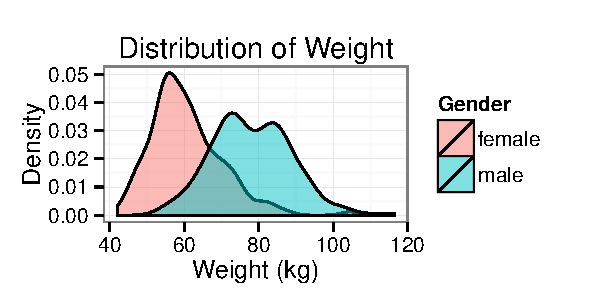
\includegraphics[width=\maxwidth]{figure/wdt} 

\end{knitrout}

\end{center}
\vspace{-20pt}
\caption{Desnsity distribution of Weight for males and females}
\label{fig:one}
\end{figure}

\begin{knitrout}
\definecolor{shadecolor}{rgb}{0.969, 0.969, 0.969}\color{fgcolor}
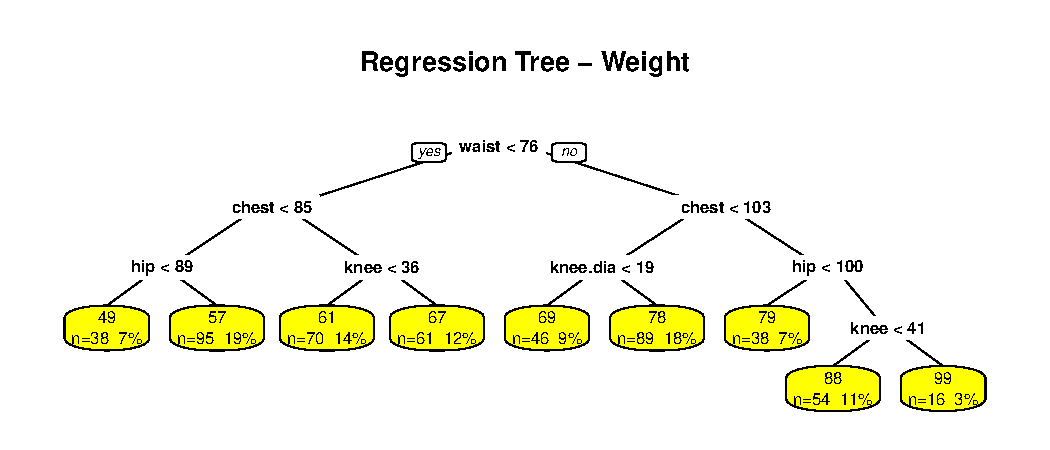
\includegraphics[width=\maxwidth]{figure/wt} 

\end{knitrout}


\subsubsection{Tree 1: Males and Females} 
To explore whether gender is an important dividing variable for the entire dataset, I first grew a regression tree with all of the data. As shown in the regression tree above, a split was not produced based on gender of the subjects. Variables used in this tree are waist girth, chest girth, hip girth, knee girth and knee diameter. \\

\pagebreak

\subsubsection{Tree 2: Males} 
Even though the full dataset did not utilize gender to partition the data, it might be informative to see if we obtain different trees by subsetting the data by gender. Next, I produced a regression tree with weight as the dependent variable for males only using all available body measurement variables. The CP tables showed us that at 5 splits we obtain a minimum relative error, therefore we were able to prune the tree to a reasonable size to avoid overfitting the data (Figure 2a). The final variables used to produce the pruned tree were hip girth and shoulder girth.

\begin{knitrout}
\definecolor{shadecolor}{rgb}{0.969, 0.969, 0.969}\color{fgcolor}\begin{kframe}
\begin{verbatim}
## 
## Regression tree:
## rpart(formula = weight ~ ., data = bodym, method = "anova")
## 
## Variables actually used in tree construction:
## [1] hip      shoulder
## 
## Root node error: 27188/247 = 110
## 
## n= 247 
## 
##      CP nsplit rel error xerror  xstd
## 1 0.552      0      1.00   1.00 0.094
## 2 0.129      1      0.45   0.47 0.049
## 3 0.069      2      0.32   0.36 0.041
## 4 0.032      3      0.25   0.31 0.030
## 5 0.025      4      0.22   0.32 0.029
## 6 0.014      5      0.19   0.31 0.028
\end{verbatim}
\end{kframe}
\end{knitrout}


\begin{figure}
\begin{knitrout}
\definecolor{shadecolor}{rgb}{0.969, 0.969, 0.969}\color{fgcolor}
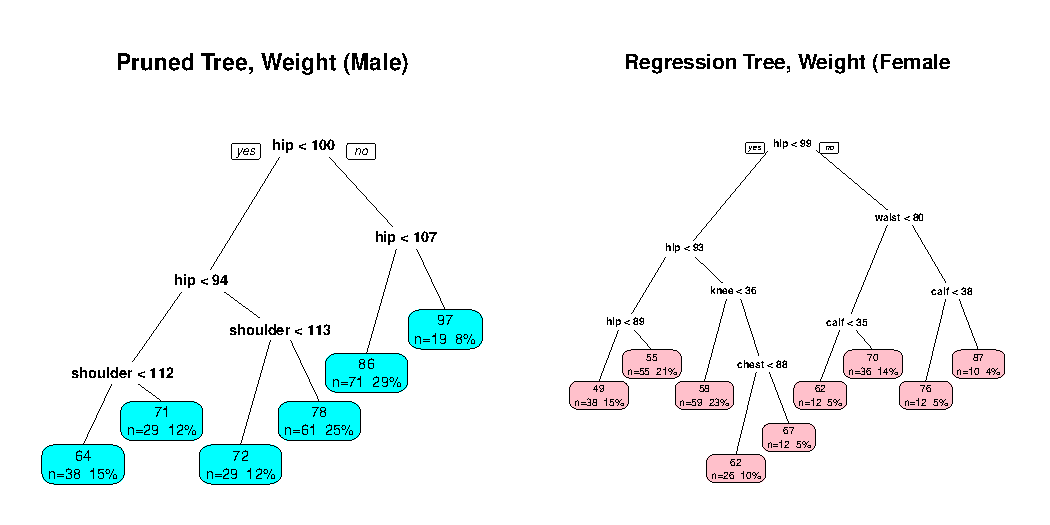
\includegraphics[width=\maxwidth]{figure/mtrees} 

\end{knitrout}

\caption{a. Pruned regression tree for male weight. b. Regression tree for female weight.}
\label{fig:two}
\end{figure}

\pagebreak

\subsubsection{Tree 3: Females} 
The regression tree for the female subset (Figure 2b) does not reach a minimum relative error before the final node and therefore did not need pruning. The variables used to produce this tree vary significantly in number and type from the male tree. They are: hip girth, knee girth, calf girth, chest girth, and waist girth. In fact, the only variable the female tree and the pruned male tree have in common is shoulder girth.

\begin{knitrout}
\definecolor{shadecolor}{rgb}{0.969, 0.969, 0.969}\color{fgcolor}\begin{kframe}
\begin{verbatim}
## 
## Regression tree:
## rpart(formula = weight ~ ., data = bodyf, method = "anova")
## 
## Variables actually used in tree construction:
## [1] calf  chest hip   knee  waist
## 
## Root node error: 23948/260 = 92
## 
## n= 260 
## 
##      CP nsplit rel error xerror  xstd
## 1 0.516      0      1.00   1.01 0.134
## 2 0.129      1      0.48   0.54 0.072
## 3 0.112      2      0.35   0.41 0.069
## 4 0.031      3      0.24   0.30 0.040
## 5 0.028      4      0.21   0.29 0.039
## 6 0.027      5      0.18   0.28 0.039
## 7 0.019      6      0.16   0.26 0.039
## 8 0.010      7      0.14   0.25 0.038
## 9 0.010      8      0.13   0.23 0.038
\end{verbatim}
\end{kframe}
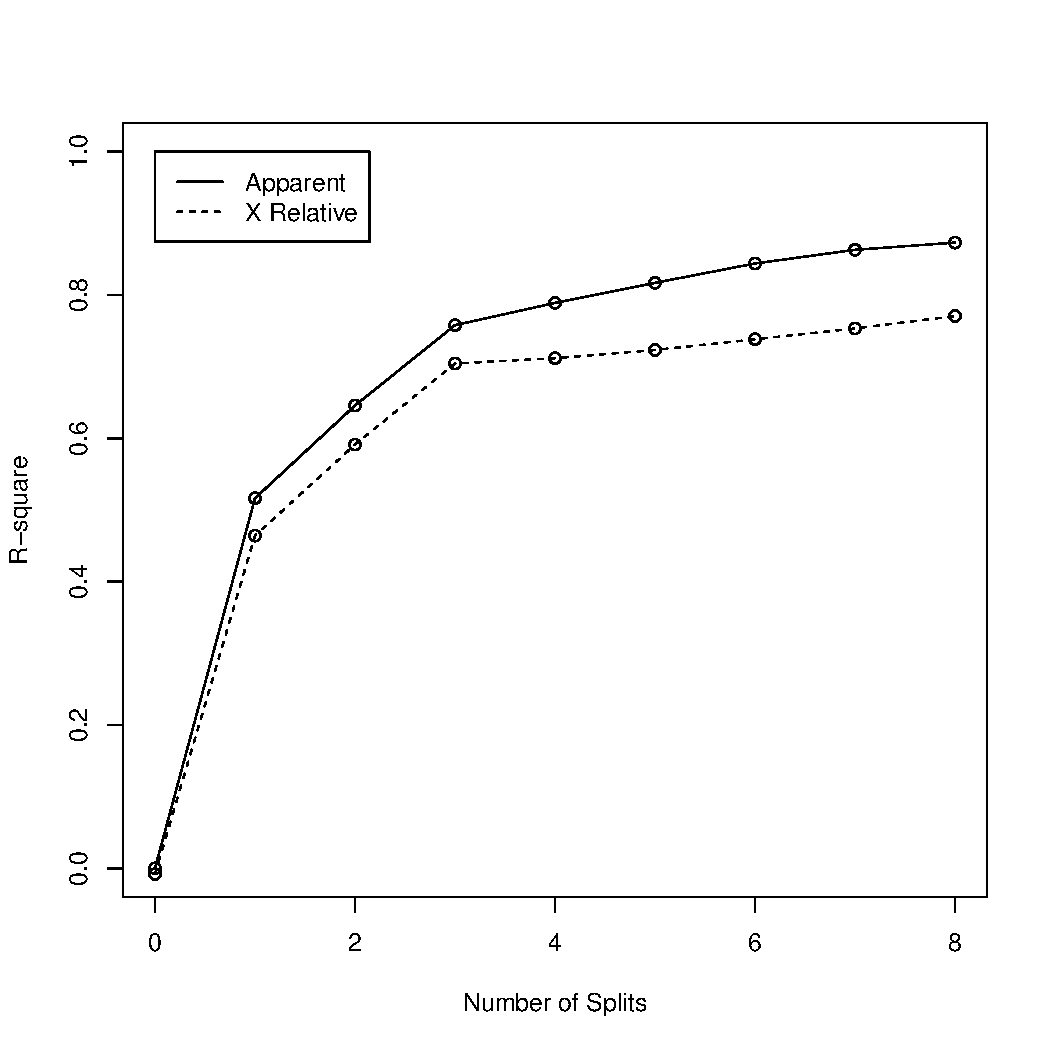
\includegraphics[width=\maxwidth]{figure/rsqf1} 

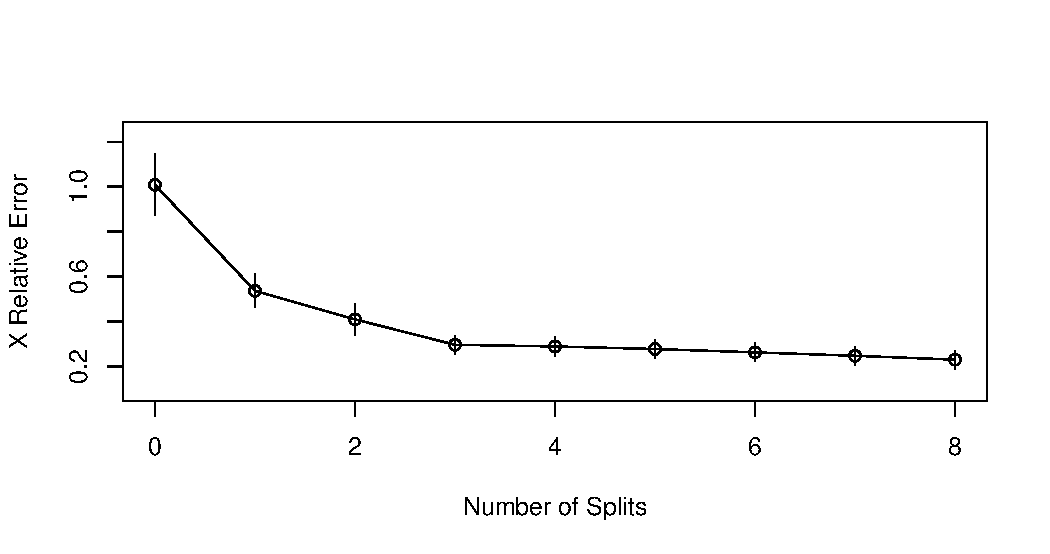
\includegraphics[width=\maxwidth]{figure/rsqf2} 

\end{knitrout}


\subsubsection{Conclusion}
While regression trees are not intended to produce a model for prediction, they can be quite useful in elucidating the most important variables for partitioning data. Here we found that these variables differed significantly between men and women, perhaps suggesting that separate models for predicting weight would be more appropriate and potentially more accurate than one general model for both genders. Further analysis would be needed to test this hypothesis, specifically model fitting and selction for subsets of the data by gender. One could then show whether these separate models have better predictive power than one combined model.
\pagebreak

%------------------------------------------------

\subsection{Model Selection (Emily)} %Emily

\subsubsection{Initial Model}

As stated previously, the initial model we are interested in fitting is of the form:\\
weight$_i = \beta_0 + \beta_1$ chest.diam$_{i} + \beta_2$ chest.dep$_{i} + \beta_3$ bitro.diam$_{i} + \beta_4$ wrist.min$_{i} + \beta_5$ ankle.min$_{i} + \beta_6$ height$_{i}$




\begin{knitrout}
\definecolor{shadecolor}{rgb}{0.969, 0.969, 0.969}\color{fgcolor}\begin{kframe}
\begin{verbatim}
## (Intercept)  chest.diam   chest.dep  bitro.diam   wrist.min 
##    -109.890       1.340       1.537       1.196       1.113 
##   ankle.min      height 
##       1.152       0.177
\end{verbatim}
\end{kframe}
\end{knitrout}


This model indicates that the expected change in weight for a 1 unit change in chest.diam, holding all other variables constant, is 1.34 lbs. The expected change in weight for a 1 unit change in chest.dep, holding all other variables constant, is 1.54 lbs., etc. Note that chest depth has the largest impact on weight. In addition to the coefficients, the R-squared value of 0.8882 implies that our model explains 88.82\% of the variation in weight and the $P$-values for each variable and for the model are significant. This model seems like a good tool to predict weight given these measurements, but are there better ones?

\subsubsection{Model Selection}

We are building a model to predict weight given various body measurements. Before running random models, we need to determine what predictors to use. The predictors needed in our models are age, height and gender. These variables contribute significantly to weight. The predictors we will allow in model selection are the initial predictors: chest diameter, chest depth and bitro diameter. In addition to these variables, pelvic bredth, shoulder, chest, waist, hip and thigh will be used. I chose to allow these predictors in my model since these are directly associated with weight (e.g. waist). However, for the other models we will fit, we will let ``R" do it's work.

\subsubsection{Criterion}

The Information Criterions we will be using to evaluate our models are Akaike Information Crierion (AIC), Bayes Information Criterion (BIC), adjusted $R^2$ and Predictive Residual Sum of Squares (PReSS). In short, AIC and BIC measure goodness-of-fit through residual sum of squares (log likelihoods) and penalizes the model size; the smaller the AIC/BIC, the better. Adjusted $R^2$ adjusts $R^2$ so that the model is penalized for adding more predictors; the higher the value of the adjusted $R^2$ the better. Finally, PRESS is a summary measure focused on prediction; the lower the value of PRESS, the better.
\begin{eqnarray*}
\text{AIC} &=& n\log \left(\dfrac{RSS}{n}\right) + 2(p +1)\\
\text{BIC} &=& n\log \left(\dfrac{RSS}{n}\right) + (p + 1) \log(n)\\
\text{adj}R^2 &=& 1 - \dfrac{n - 1}{n - p - 1}(1 - R^2)\\
\end{eqnarray*}
\begin{eqnarray*}
\text{PRESS} &=& \sum{\left(\dfrac{\hat{\epsilon}_i}{1 - h_{ii}}\right)^2}
\end{eqnarray*}

\subsubsection{Methods in R}

There are multiple methods built into different packages in R for Model Selection. To illustrate these, we will use the variables:  height, wrist.min, ankle.min and chest.



\\

\textbf{stepAIC()}\\

The R function found in the package ``MASS" called ``stepAIC()" performs stepwise model selection by AIC. This will output the initial model and the final model (model of best fit determined by this method), and the steps taken. In the output below we can see that this method suggests using a different model that doesn't contain wrist.diam.\\




\texttt{Initial Model: weight ~ height + wrist.diam + ankle.diam + chest\\
Final Model: weight ~ height + ankle.diam + chest\\
\begin{tabular}{r r r r r r r}
        &  Step & Df & Deviance & Resid. Df & Resid. Dev & AIC \\
1  &            &      &        &  502 &  13294.14 & 1666.150 \\
2 & - wrist.diam & 1 & 47.90427 & 503 &   13342.05 & 1665.974
\end{tabular}
}

\\

\textbf{leaps()}\\

The R package ``leaps" contains a function ``regsubsets()". This method performs an exhaustive search of models and plots the $R^2$ criterion by variables and subset size. The class ``summary.regsubsets" outputs an object with multiple elements, including adjusted $R^2$ and BIC. Furthermore, the plots below plot the  
BIC and Adjusted $R^2$ values against each subset of variables. 

\begin{knitrout}
\definecolor{shadecolor}{rgb}{0.969, 0.969, 0.969}\color{fgcolor}
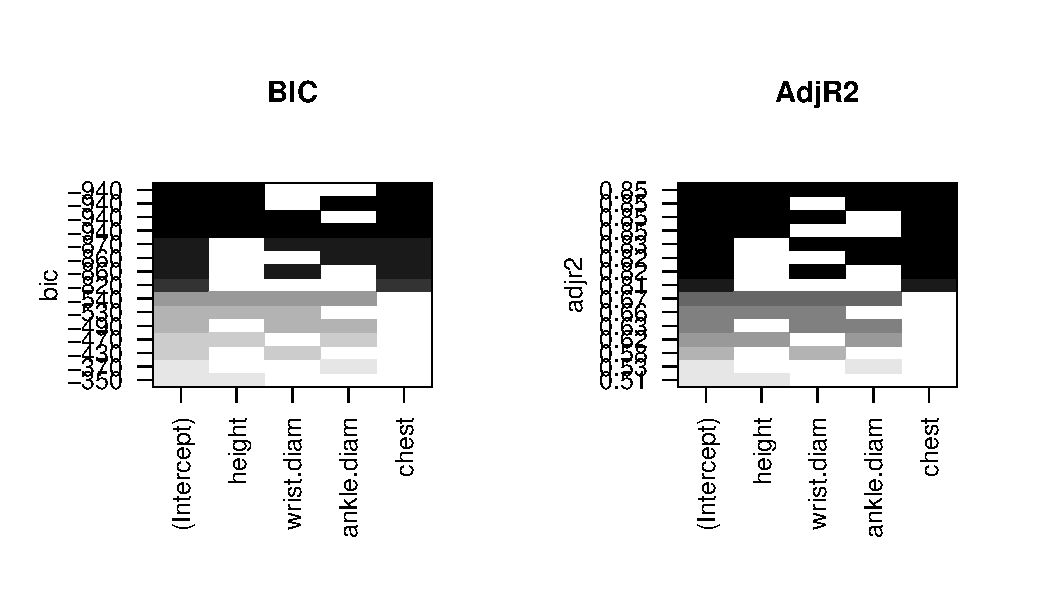
\includegraphics[width=\maxwidth]{figure/leap} 

\end{knitrout}


In these plots, for example, the BIC plot is implying the best model is using height and chest as predictors. On the other hand, the AdjR2 plot is saying all variables give the best fit. Using both of these plots together, one might conclude height, ankle.diam and chest would be the best fit. This conclsion agrees with our analysis using stepAIC.

\subsubsection{Model Selection in Action}




The Model Selection Lab will explain how to obtain the models summarized in Table 1.     

\textbf{Table 1}\\

\begin{center}
\begin{tabular}{|r|c|c|c|c|r|}
  \hline
MLR\# & AIC & BIC & PRESS & Adjusted $R^2$ & Method \\ 
  \hline
all & 2216 & 2326 & 2384 & 0.9753 & \text{all variables  from dataset used} \\ \hline
i & 2970 & 3004 & 10405 & 0.8869 & \text{suggested by paper} \\ \hline
1 & 2256 & 2319 & 2560 & 0.9727 & \text{suggested by paper}\\ \hline
2 & 2402 & 2441 & 3408 & 0.9632 & \text{my model}\\ \hline
3 & 2206 & 2282 & 2329 & 0.9754 & \text{stepAIC} \\ \hline
4 & 2195 & \textcolor{blue}{2271} & \textcolor{blue}{2281} & \textcolor{blue}{0.9759} & \text{stepAIC and adjustments} \\ \hline
5 & 2207 & 2292 & 2335 & 0.9755 &\text{leaps (adj} R^2) \\ \hline
6 & \textcolor{red}{2189} & 2278 & \textcolor{red}{2255} & \textcolor{red}{0.9764}  & \text{leaps(adj} R^2) \text{and adjustments}\\ \hline
7 & 2213 & 2272 & 2353 & 0.9749 & \text{leaps(BIC)} \\ \hline
8 & \textcolor{blue}{2205} & \textcolor{red}{2264} & 2316 & 0.9753 & \text{leaps(BIC) and adjustments}\\ \hline
\end{tabular}
\end{center}

Base on Table 1, we can see that each criteria yields different results. It is up to our discretion to choose a model. \textcolor{red}{Red} corresponds to the best value, of all 10 models, for that criteria, \textcolor{blue}{blue} is the second best. Since AIC and PRESS are lowest in MLR6, the adjusted $R^2$ is the largest, and the BIC is close to the best and second best values, I would choose MLR6 as the model of best fit. MLR6 is of the form:\\ 

weight$_i = \beta_0 + \beta_1$ pelvic.bredth$_{i} + \beta_2$ bitro.diam$_{i} + \beta_3$ chest.dep$_{i} + \beta_4$ chest$.diam_{i}$ + \beta_5$ elbow.diam$_{i} + \beta_6$ knee.diam$_{i}$ + 
\beta_7$ shoulder$_{i}$ + \beta_7$ chest$_{i}$ + \beta_8$ waist$_{i}$ + \beta_9$ hip$_{i}$ + \beta_{10}$ thigh$_{i}$ + \beta_{11}$ bicep_{i} + \beta_{12}$ forearm_{i} + \beta_{13}$ knee_{i} + \beta_{14}$ calf_{i} +\beta_{15}$ age_{i} + \beta_{16}$ height_{i} + \beta_{17}$ gender_{i} + \beta_{18}$ height$^2_{i}$. \\

Note in Table 1 the first and second lowest values for AIC, BIC and Press, and the first and second highest values for Adjusted $R^2$ were for stepAIC with adjustments and leaps with adjustments.

\subsubsection{Conclusion}
Model Selection truely is an art form. R can mechanically run through steps, interactions, combinations, etc. However, R cannot subjectively look at the variables to determine the absolute best model. To acheive the model of best fit, a combination of methods and human adjustment is necessary.

\newpage

%------------------------------------------------

\subsection{Resampling Inference and  Bootstrapping} %Nick

%------------------------------------------------

\subsection{Logistic Regression and Ada-boosting} %Yiding


\end{document}
